\section{Results}

% Figure 1: overview, from fig1_overview_standalone.pdf (built by the Makefile).
\begin{figure*}[t]
\centering
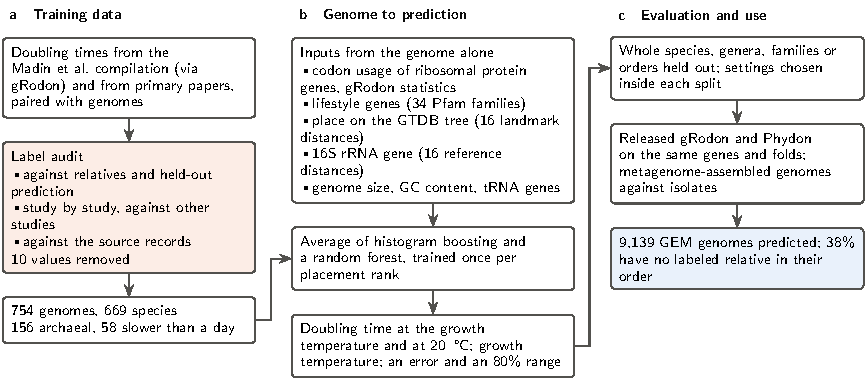
\includegraphics[width=0.82\textwidth,alt={Flow diagram in three columns. Training data: doubling times from the Madin compilation and primary papers, a label audit that removed values which are not maximal growth rates, and the final training set. Genome to prediction: inputs computed from the genome, a model averaging histogram boosting and a random forest, and three predicted quantities with errors and ranges. Evaluation and use: lineage-held-out evaluation, comparison with released tools and with metagenome-assembled genomes, and predictions for the GEM catalog.}]{fig1_overview_standalone}
\caption{Overview. (a) Growth rates were collected and audited for values that are not maximal growth rates. (b) Every input
is computed from the genome, so the same model applies to isolates and to metagenome-assembled genomes. (c) Accuracy is
measured with whole lineages held out, which is the situation of most environmental genomes, and the measured error at each
level of novelty is attached to every prediction.}
\label{fig:overview}
\end{figure*}


\begin{table}[t]\centering\footnotesize\setlength{\tabcolsep}{3pt}
\caption{Training data after the label audit. Rows are genomes with a measured doubling time; slow means a doubling time above 24 h; gene features are available where the genes could be predicted and annotated. The audit removed 10 values (Supplementary Table~\ref{S-tab:exclusions}). Genome size, GC content and tRNA count are computed from the genome, except in the rows marked $^{a}$, which take them from the compilation.}\label{tab:data}
\begin{tabular}{lrrrrr}
\toprule
Source & Genomes & Species & Archaea & Slow & Gene features \\
\midrule
gRodon's growth table & 294 & 209 & 0 & 14 & 294 \\
Madin et al., with traits$^{a}$ & 291 & 291 & 99 & 18 & 279 \\
Madin et al., genome only & 161 & 161 & 53 & 20 & 161 \\
Literature strains & 8 & 8 & 4 & 6 & 8 \\
\midrule
Total & 754 & 669 & 156 & 58 & 742 \\
\bottomrule
\end{tabular}
\end{table}


\subsection{One study was enough to create a biological effect}
After the audit, the training set holds \NGenomes genomes from \NSpecies species; \NArchaea are archaeal and \NSlow double
less than once a day (Table~\ref{tab:data}). We removed \NExcluded values from \NExcludedSourcesWord sources, each only after a
second source for the species, or the study itself, showed that it was not a maximal growth rate at the stated temperature
(Supplementary Table~\ref{S-tab:exclusions}).

The case that shaped the audit involved \NExcludedKevbrinaWord methanotrophs. The compilation gives them doubling times of
\KevLabelMin to \KevLabelMax hours, taken from a study of growth at low temperature \citep{kevbrina2001}. The records of the
same study in the source compilation say \KevRecordMin to \KevRecordMax hours, about \KevRatio times more, which points to a
unit slip somewhere between the two. Neither version is a maximal growth rate. Yet with relatedness controlled, these
\NExcludedKevbrinaWord values alone make carriers of methane or ammonia monooxygenase look \KevFoldWith-fold slower (95\%
interval \KevLowWith to \KevHighWith, adjusted $p=\KevPWith$), exactly the kind of effect one would cite as evidence that
organisms on thin energy budgets grow slowly. Without them the estimate is \KevFoldWithout-fold (\KevLowWithout to
\KevHighWithout, adjusted $p=\KevPWithout$). Because the four values came from one study and agreed with each other, every
methanotroph genus looked slow, and no comparison with relatives could have caught it.

That is why the audit compares each study with evidence from other studies. With the exclusions switched off, the
study-level check recovers \PosCtrlCaughtWord of the \PosCtrlNWord values we had removed before it existed. The one it misses,
a lag-phase measurement of \textit{Klebsiella oxytoca}, is the only value from its study and was caught by the comparison with
relatives instead. On the current labels the check flags \NStudiesFlagged of \NStudiesCompared studies, and we found a
plausible reason for each when we read them, such as rich-medium rates of haloarchaea at their optimum. Most studies contribute
a single value, so the audit lowers the error rate of the labels but cannot certify them.

\begin{figure*}[t]
\centering
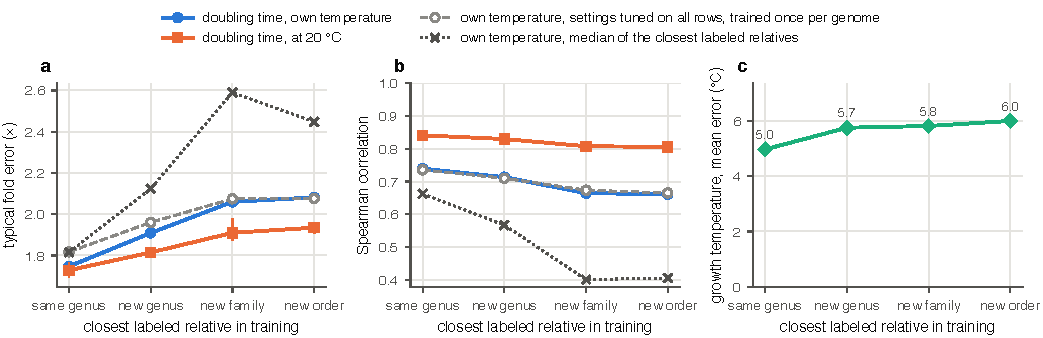
\includegraphics[width=\textwidth,alt={Three line panels against the closest labeled relative (same genus, new genus, new family, new order). Panel a: typical fold error of the doubling time rises with novelty and is lower for the 20 C value; the median of the closest labeled relatives is close to the model with species held out and clearly worse with families or orders held out. Panel b: Spearman correlation falls with novelty. Panel c: mean absolute error of growth temperature rises slightly with novelty.}]{fig2_accuracy}
\caption{Accuracy by the closest labeled relative of a genome, with that whole level held out (settings chosen inside each
split, \NSeedsHeadline seeds; bars span the seeds). (a) Typical fold error of the doubling time at the growth temperature and
at \TRefC\,\textdegree C. The dashed line is the same model with settings chosen on all labeled genomes and each genome
trained once, the scheme behind the error table released with the predictions; the dotted line predicts each genome by
the median label of its closest labeled relatives. (b) Spearman correlation. (c) Mean absolute error
of the growth temperature.}
\label{fig:accuracy}
\end{figure*}

\subsection{Accuracy falls with lineage novelty, and each prediction can carry its error}
We held out whole species groups, genera, families or orders, so that every test genome has its closest labeled relative at
a known level, and chose the model settings inside each split (Figure~\ref{fig:accuracy}, Supplementary
Table~\ref{S-tab:accuracy}). With a relative in the same genus, the predicted doubling time is typically off by
\ErrSameGenus-fold (95\% interval \CIErrLoSameGenus to \CIErrHiSameGenus; Spearman \RhoSameGenus). With the whole order held
out it is off by \ErrNewOrder-fold (\CIErrLoNewOrder to \CIErrHiNewOrder; Spearman \RhoNewOrder). Most of the loss happens
before the family level. The doubling time at \TRefC\,\textdegree C is predicted better at every level (\ErrRefSameGenus- to
\ErrRefNewOrder-fold), because much of the spread in doubling times comes from temperature, which the model itself predicts to
within \TempMAESameGenus to \TempMAENewOrder\,\textdegree C on average.

\paragraph{Against taxonomy alone.} A simple alternative predicts each genome by the median label of its closest labeled
relatives. When only the species is held out, this is nearly as good as the model (\BaseRelErrSameGenus-fold; the interval of
the difference, \CIDiffLoSameGenus to \CIDiffHiSameGenus, includes zero), although it ranks genomes worse (Spearman
\BaseRelRhoSameGenus against \RhoSameGenus). As relatives become distant it falls well behind: \BaseRelErrNewFamily- and
\BaseRelErrNewOrder-fold with families or orders held out, against \ErrNewFamily- and \ErrNewOrder-fold for the model.
Trained on labels shuffled across genomes, the model is no better than the median (\ShuffleErrSpecies-fold, Spearman
\ShuffleRhoSpecies), so the evaluation itself creates no accuracy.

\paragraph{Robustness.} Three further checks, run with the deployed settings over \TenNSeeds splits, leave these conclusions
intact (Supplementary Table~\ref{S-tab:robust}). Once the genus is held out, the model beats the relatives' median in
\TenModelWinsDeepMin of \TenNSeeds splits at every level (per genome $p$ \TenPGenomeDeepMax); with only the species held out
the two stay close (\TenModelErrSpecies- against \TenBaseErrSpecies-fold) and the model still ranks better. One input,
gRodon's own estimate, comes from a regression whose coefficients saw our species; refitting that regression inside each
split raises the error by at most \RefitMaxDiff, which bounds any leakage through it. Dropping the \FlagNLabels labels from
studies that the audit flagged but kept lowers the error on the remaining genomes slightly (\FlagErrOrder- against
\FlagFullErrOrder-fold with orders held out).

\paragraph{Training scheme.} Entering each training genome once for each of its four tree placements lowers the error with
the species held out from \FixedErrSameGenus- to \CoarseErrSameGenus-fold. Choosing the settings inside each split changes
the error at the growth temperature by at most \SelectMaxDiff, but at \TRefC\,\textdegree C it is slightly worse with orders held out
(\ErrRefNewOrder- against \FixedErrRefNewOrder-fold), so the released \TRefC\,\textdegree C errors are slightly optimistic.

\paragraph{Slow growers and archaea.} Slow growth is ranked better than it is predicted. The area under the curve for a
doubling time above a day is \AucSameGenus with the species held out and \AucNewOrder with orders held out, but predictions
are pulled toward the middle of the range. With the species held out, only \SlowCalledSpecies of \SlowTotalSpecies slow
species groups get a prediction above a day (\SlowCalledTrueSpecies correctly); with orders held out the count drops to \SlowCalledOrder. The typical
error of slow growers is \ErrSlowSpecies- to \ErrSlowOrder-fold, almost always toward faster growth. A prediction above a day
is therefore strong evidence of slow growth, while a short one is weak evidence against it. Archaea are also predicted less
well than bacteria (\ErrArchOrder- against \ErrBactOrder-fold with orders held out).

\paragraph{Ranges and the probability of slow growth.} Ranges set by novelty level alone contain \CovNovAllSpecies\% of
measured values with species held out and \CovNovAllOrder\% with orders held out, but only \CovNovArchOrder\% for archaea from held-out
orders. Setting them by novelty level and domain restores at least \CovDomArchMin\% for archaea, and these are the ranges we
release. No range built from the inputs can hold for organisms that are slow in truth (\CovDomSlowMin\% to
\CovDomSlowMax\%), since the model cannot single them out. For that question we release a probability of growing slower than
a day. It ranks genomes well (AUC \SlowProbAucSpecies and \SlowProbAucOrder) and is calibrated (error at most
\SlowProbECEMax), but it is modest: in the fifth of genomes with the highest probability, \SlowProbTopSpecies\% are slow,
against \SlowBaseRate\% overall.

\begin{table}[t]\centering\footnotesize\setlength{\tabcolsep}{3pt}
\caption{The released gRodon and Phydon against this model on the same 680 genomes, genes and species-held-out folds (mean of 3 seeds; this model built inside each split as in Algorithm~\ref{alg:nested}). T: the measured growth temperature is given as an input. Error: typical fold error; $\rho$: Spearman correlation; AUC: for a doubling time above a day. Wins: genomes, of those both methods predict, for which this model (without or with the temperature) has the smaller absolute log error, averaged over seeds, with the paired Wilcoxon $p$. Phydon placed 665 genomes.}\label{tab:released}
\begin{tabular}{@{}lccccc@{\hspace{4pt}}c@{}}
\toprule
& & & & & \multicolumn{2}{c}{Wins of this model} \\
\cmidrule(lr){6-7}
Method & T & Error & $\rho$ & AUC & without T & with T \\
\midrule
This model & no & 1.76 & 0.72 & 0.85 & -- & -- \\
This model & yes & 1.70 & 0.76 & 0.87 & -- & -- \\
gRodon & no & 2.40 & 0.52 & 0.75 & 424/680 ($<$0.001) & 453/680 ($<$0.001) \\
gRodon & yes & 1.92 & 0.73 & 0.84 & 349/680 (0.07) & 383/680 ($<$0.001) \\
Phydon & yes & 1.85 & 0.70 & 0.81 & 347/665 (0.11) & 355/665 ($<$0.001) \\
\bottomrule
\end{tabular}
\end{table}


\subsection{Against gRodon and Phydon, the model helps most when the temperature is unknown}
We ran the released gRodon \citep{weissman2021} and Phydon \citep{xu2025} on the same \RelN genomes, genes and
species-held-out folds as our model, after removing each fold's test species from Phydon's own training table (Methods). Both
tools need the measured growth temperature. Given it too, our model has a typical error of \RelOursTempErr-fold, against
\RelGRodonErr-fold for gRodon and \RelPhydonErr-fold for Phydon (Table~\ref{tab:released}), with a higher Spearman correlation
and area under the curve. It is better in every seed and, per genome, against both tools ($p=$\,\PairTempGRodonP and
\PairTempPhydonP).

An uncultured genome comes without a temperature, and without it gRodon's error rises to \RelGRodonNoTempErr-fold. Our model,
which predicts the temperature itself, keeps an error of \RelOursErr-fold. That is lower than either tool's error with the
temperature, in every seed, but per genome the difference is not significant (\PairGRodonBetter of \PairGRodonN genomes
favour our model against gRodon, $p=\PairGRodonP$; \PairPhydonBetter of \PairPhydonN against Phydon, $p=\PairPhydonP$).
Without the temperature, then, the model matches the released tools given it rather than beating them. The tools keep one
further advantage in this comparison: their parameters were fitted on data that include our test species.

With whole orders held out (and cut from Phydon's training table), Phydon's error rises to \RelOrdPhydonErr-fold, while
gRodon, which uses no relatives, stays at \RelOrdGRodonErr-fold given the temperature. Our model then ties with gRodon given
the temperature (\RelOrdOursTempErr-fold, $p=\PairOrdTempGRodonP$) and trails it without (\RelOrdOursErr-fold,
$p=\PairOrdGRodonP$), but stays ahead of gRodon without the temperature (\RelOrdGRodonNoTempErr-fold,
$p$\,\PairOrdGRodonNoTempP), the case of an uncultured genome.

\subsection{On species outside both training compilations}
To test the released model on labels it had never seen, we collected \ExtNCurated doubling times from species descriptions,
each the fastest growth in pure culture, for species absent from the compilation of \citet{madin2020} (by NCBI taxonomy
identifier, which survives renaming) and from our labels, with no training genome in their GTDB species (Methods;
Supplementary Table~\ref{S-tab:external}). \ExtN have usable genomes, \ExtNNewOrder without a labeled relative in their
order. The model is off by \ExtModelErr-fold (95\% interval over genera \ExtModelLo to \ExtModelHi, Spearman \ExtModelRho),
against \ExtBaseErr-fold for the relatives' median and \ExtGRodonErr-fold for gRodon without a temperature, and is closer for
\ExtBetterBase and \ExtBetterGRodon of the \ExtN species ($p=\ExtPBase$ and \ExtPGRodon). The error grows from
\ExtModelErrSameGenus-fold within a labeled genus to \ExtModelErrNewOrder-fold in a new order, more than in
cross-validation. The ranges are too narrow here, holding \ExtCoverage\% of the values instead of 80\% ($p=\ExtCoverageP$)
and \ExtCoverageSlowIn of the \ExtNSlow species slower than a day; the slow-growth probability ranks those \ExtNSlow well
(AUC \ExtSlowAuc), but none is predicted to take more than a day.

\subsection{What the accuracy comes from}
\begin{table*}[t]\centering\footnotesize\setlength{\tabcolsep}{3.5pt}
\caption{What each part contributes. Each row changes one thing in the final model and gives the mean change over 10 seeds, with the number of seeds in which the variant did better in brackets; $^{*}$ paired Wilcoxon $p<0.05$. Typical error is the fold error of the median genome (lower is better); AUC ranks genomes slower than a day. All variants are scored on the same genomes and folds, with the deployed settings and each genome entered once. The seeds reshuffle the same genomes, so $p$ measures how consistent a change is across splits, not independent replication. $^{\dagger}$The earlier learner (gradient boosting, 200 trees of depth 3) against the tuned average, both with settings chosen inside each split (5 seeds).}\label{tab:ablations}
\begin{tabular}{lcccccc}
\toprule
& \multicolumn{3}{c}{Species held out} & \multicolumn{3}{c}{Orders held out} \\
\cmidrule(lr){2-4} \cmidrule(lr){5-7}
& Typical error ($\times$) & Spearman & AUC, slow & Typical error ($\times$) & Spearman & AUC, slow \\
\midrule
final model & 1.819 & 0.740 & 0.838 & 2.093 & 0.654 & 0.803 \\
\midrule
without gRodon statistics & +0.110$^{*}$ (0/10) & $-$0.044$^{*}$ (0/10) & $-$0.010$^{*}$ (0/10) & +0.295$^{*}$ (0/10) & $-$0.080$^{*}$ (0/10) & $-$0.045$^{*}$ (0/10) \\
without lifestyle genes & +0.005 (4/10) & $-$0.002$^{*}$ (1/10) & 0.000 (3/10) & $-$0.020 (6/10) & +0.005$^{*}$ (8/10) & +0.002$^{*}$ (7/10) \\
without any gene features & +0.274$^{*}$ (0/10) & $-$0.078$^{*}$ (0/10) & $-$0.033$^{*}$ (0/10) & +0.551$^{*}$ (0/10) & $-$0.195$^{*}$ (0/10) & $-$0.076$^{*}$ (0/10) \\
without 16S & $-$0.002 (7/10) & +0.002$^{*}$ (8/10) & 0.000 (6/10) & 0.000 (6/10) & 0.000 (7/10) & $-$0.010$^{*}$ (1/10) \\
without GTDB phylogeny & +0.026$^{*}$ (1/10) & $-$0.008$^{*}$ (0/10) & +0.002 (7/10) & $-$0.023$^{*}$ (8/10) & +0.002 (7/10) & +0.006$^{*}$ (10/10) \\
without the added species & +0.040$^{*}$ (0/10) & $-$0.009$^{*}$ (0/10) & $-$0.003$^{*}$ (1/10) & +0.040$^{*}$ (0/10) & $-$0.004 (3/10) & $-$0.006$^{*}$ (2/10) \\
with energy-metabolism genes & +0.002 (4/10) & 0.000 (5/10) & +0.001 (7/10) & +0.013$^{*}$ (3/10) & $-$0.001 (4/10) & $-$0.001 (4/10) \\
with predicted growth temperature & $-$0.015 (6/10) & $-$0.001 (4/10) & 0.000 (5/10) & $-$0.015$^{*}$ (8/10) & +0.004$^{*}$ (8/10) & +0.002 (7/10) \\
earlier learner, nested$^{\dagger}$ & & & & +0.015 (1/5) & $-$0.021 (0/5) & $-$0.012 (0/5) \\
\bottomrule
\end{tabular}
\end{table*}


The accuracy comes from the genes (Table~\ref{tab:ablations}; deployed settings, one placement per genome). Without gRodon's
codon usage statistics the error rises from \AblFinalErrSpecies- to \AblGStatErrSpecies-fold with the species held out and
from \AblFinalErrOrder- to \AblGStatErrOrder-fold with orders held out; without any gene features it rises to
\AblGenesErrSpecies- and \AblGenesErrOrder-fold, worse in all \NSeedsAblation seeds. The species we added to the earlier
training data help at both levels. The GTDB phylogeny helps only when a relative in the same genus is labeled, as one would
expect when the closest relatives are far away. The 16S inputs leave the typical error unchanged; with orders held out they
add a little to the ranking of slow growers (AUC \AblFinalAucOrder against \AblSixteenAucOrder without them). Energy-metabolism genes do not help, and a predicted growth temperature as an extra input gains too
little to justify a second model. The tuned average of two learners improved only slightly on the earlier single model
(\TuneErrBefore- to \TuneErrAfter-fold with orders held out).

\paragraph{A learned representation.} A generic protein language model does as well as our hand-built features. A ridge
probe on ESM-2 embeddings \citep{lin2023} of each genome's ribosomal proteins and \EsmNOther other proteins reaches
\EsmProbeErrSameGenus-fold with species held out and \EsmProbeErrNewOrder-fold with orders held out, against
\EsmFeatErrSameGenus- and \EsmFeatErrNewOrder-fold for the features (per genome $p=\EsmProbePSameGenus$ and
\EsmProbePNewOrder). The two are complementary: adding \EsmPCComb principal components of the embeddings to the features
lowers the error to \EsmCombErrSameGenus- and \EsmCombErrNewOrder-fold ($p=$\,\EsmCombPSameGenus and \EsmCombPNewOrder;
Supplementary Table~\ref{S-tab:esm}). The released predictions do not use embeddings yet.

\paragraph{A trap in the 16S input.} Most labeled species first had their 16S gene retrieved from NCBI by name, while a GEM
genome's gene is cut from the genome itself; for \SixteenFarther labeled genomes the NCBI copy was farther from the
genome's own gene than from another species. A model trained on NCBI copies and given genome copies, as the GEM genomes had
been, did worse in every seed (\SixteenErrMixedOrder- against \SixteenErrNcbiOrder-fold with orders held out). All results
here use the copy cut from the genome wherever barrnap finds one (\SixteenNGenomeCopy genomes).

\begin{figure*}[t]
\centering
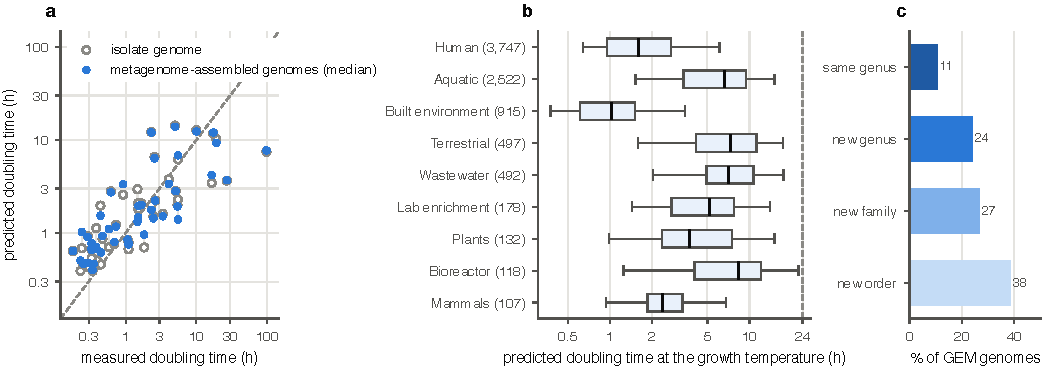
\includegraphics[width=\textwidth,alt={Panel a: scatter of predicted against measured doubling time, with isolate and metagenome-assembled predictions for each species joined by lines, lying close together. Panel b: box plots of predicted doubling time of GEM genomes by habitat. Panel c: bar chart of the share of GEM genomes by closest labeled relative.}]{fig4_mags_gem}
\caption{From isolates to the GEM catalog. (a) Predicted against measured doubling time for \MagNSpecies species held out of
training, predicted from the isolate genome (open) and from the species' metagenome-assembled genomes in GEM (filled, median
over the assembled genomes of a species); lines join the two predictions. (b) Predicted doubling times of GEM genomes by
habitat, for habitats with at least 100 genomes (boxes: quartiles; whiskers: 5th and 95th percentiles; dashed line: one day).
(c) Closest labeled relative of the GEM genomes.}
\label{fig:mags}
\end{figure*}

\subsection{Predictions transfer to metagenome-assembled genomes}
The GEM catalog contains \MagNGenomes assembled genomes of \MagNSpecies species with a measured growth rate. With each species
held out of training, predictions from its assembled genomes are off by \MagErr-fold (95\% interval \CIMagErrLo to
\CIMagErrHi), against \MagIsoErr-fold from its isolate genome; the interval of the difference (\CIMagDiffLo to \CIMagDiffHi)
includes zero (Figure~\ref{fig:mags}a). The two predictions sit close together, a median of \MagGap-fold apart, and for
\MagGapSmaller of the \MagNSpecies species the gap is smaller than the error of the isolate prediction itself. Most of the
error on assembled genomes is the error the model makes on any new species, not a cost of assembly.

\begin{figure}[t]
\centering
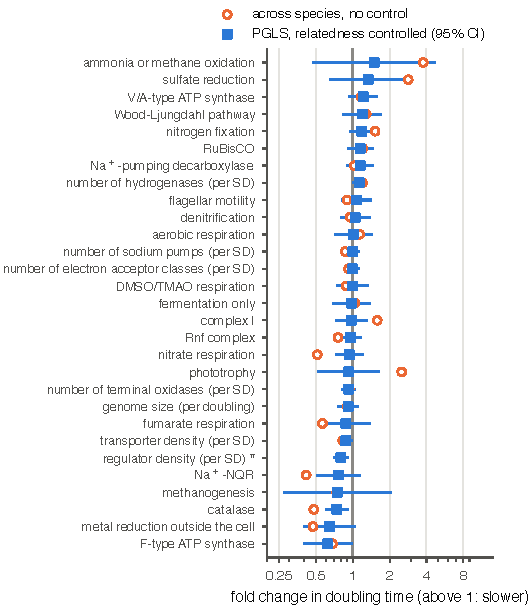
\includegraphics[width=\columnwidth,alt={Forest plot of fold change in doubling time for each gene-content input, without and with phylogenetic control; with control, most intervals cross one and no energy-metabolism input remains significant after adjustment for the number of inputs.}]{fig5_lifestyle}
\caption{Gene content and doubling time across \PglsNGroups species groups, without control for relatedness (open circles)
and with phylogenetic generalized least squares (squares, 95\% intervals), with growth temperature and domain as
covariates. Effects are fold changes for carrying a gene, per standard deviation of a count or density, or per doubling of
genome size. $^{*}$Adjusted $p<0.05$.}
\label{fig:lifestyle}
\end{figure}

\subsection{Slow growers carry fewer transporter genes, not an energy-poor metabolism}
Doubling time is strongly patterned by relatedness (Pagel's $\lambda=\PglsLambda$ over \PglsNGroups species groups), so a raw
comparison across species counts one slow clade many times over. Across species, several energy-related inputs do look
associated with growth rate: phototrophy, sulfate reduction and monooxygenases with slower growth, nitrate respiration and the
Na$^+$-translocating NADH dehydrogenase with faster growth (Figure~\ref{fig:lifestyle}). Once relatedness is controlled, none
of the inputs that describe how an organism makes energy is associated with its doubling time (adjusted $p\ge\PglsEnergyMinP$
for all of them).

Two inputs about how an organism senses and draws on its surroundings remain. A higher density of regulator genes goes with
faster growth (\PglsRegFold-fold per standard deviation, adjusted $p=\PglsRegP$), but the association rests on the
Pseudomonadota and disappears without them. The clearest signal for growing slower than a day is a low density of transporter
genes: the odds of being slow fall to \SlowTransporterOR per standard deviation more transporters ($p=$\,\SlowTransporterP),
with \KEigen phylogenetic eigenvectors as covariates, and the result holds with half or one and a half times as many.

\subsection{Growth rates for the GEM catalog}
Across the \NGEMPredicted high-quality GEM genomes, the median predicted doubling time at the growth temperature is
\GEMMedianHours hours (Figure~\ref{fig:mags}b). Only \GEMNSlow genomes (\GEMShareSlow\%) are predicted to double less than
once a day, most of them \GEMSlowTopOrder (\GEMSlowTopOrderN) and ammonia-oxidizing archaea of the \GEMSlowSecondOrder
(\GEMSlowSecondOrderN). Genomes from the human body (median \GEMMedianHuman hours, \GEMNHuman genomes) and the built
environment (\GEMMedianBuilt hours) are predicted to grow faster than those from aquatic (\GEMMedianAquatic hours) and
terrestrial habitats (\GEMMedianTerrestrial hours). The habitats also differ in how well labeled relatives cover them:
\GEMNewOrderHuman\% of human-associated genomes have no labeled relative in their order, against \GEMNewOrderAquatic\% of
aquatic and \GEMNewOrderTerrestrial\% of terrestrial ones (Figure~\ref{fig:mags}c). Predictions for environmental habitats
therefore carry the larger errors of Figure~\ref{fig:accuracy}, and each is released with its novelty level, error and range.
